\documentclass[3p, sort&compress]{elsarticle}
\usepackage{amsmath}
\usepackage{amssymb}
\usepackage{amsthm}
\usepackage{amsfonts}
\usepackage{amsbsy}
\usepackage{amstext}
\usepackage{amsfonts}
\usepackage{amstext}
\usepackage{mathrsfs}
\usepackage{graphpap}
\usepackage{graphics,graphicx}
\usepackage[utf8]{inputenc}
\usepackage{subcaption}
\usepackage{multicol}
\usepackage{booktabs}
\usepackage{array}
\usepackage{siunitx}
\usepackage{hyperref}
\usepackage[section]{placeins}
\usepackage{xargs}
\usepackage[pdftex,dvipsnames]{xcolor}
\usepackage[colorinlistoftodos,prependcaption,textsize=tiny]{todonotes}
\graphicspath{{./plotly_chart_studio_figures/}}
\graphicspath{{./figures/}}
%
%
\newcommandx{\unsure}[2][1=]{%
    \todo[
        linecolor=red,
        backgroundcolor=red!25,
        bordercolor=red, #1]{#2}
}%
\newcommandx{\change}[2][1=]{%
    \todo[
        linecolor=blue,
        backgroundcolor=blue!25,
        bordercolor=blue, #1]{#2}
}
\newcommandx{\info}[2][1=]{%
    \todo[
        linecolor=OliveGreen,
        backgroundcolor=OliveGreen!25,
        bordercolor=OliveGreen, #1]{#2}
}
\newcommandx{\improvement}[2][1=]{
    \todo[linecolor=Plum,
        backgroundcolor=Plum!25,
        bordercolor=Plum,#1]{#2}
}
\newcommandx{\thiswillnotshow}[2][1=]{\todo[disable,#1]{#2}}
\hypersetup{colorlinks = true, allcolors = blue}
\usepackage[nameinlink,noabbrev]{cleveref}
\newcommand{\R}{\mathbb{R}}
\newcommand{\e}{\varepsilon}
\newcommand{\f}{\mathfrak{F}}
\newcommand{\Q}{\mathbb{Q}}
\newcommand{\N}{\mathbb{N}}
\newtheorem{teor}{Theorem}
\newtheorem{lemma}{Lemma}
\usepackage[toc,page]{appendix}
%
%
\begin{document}
    \begin{frontmatter}
        \title{
            Optimal vaccination preventive policies for COVID-19\\
        }
        \author[add:conacyt_unison]{%
            Sa\'ul D\'iaz-Infante%
            \corref{corresponding_author}%
        }%
        \ead{saul.diazinfante@unison.mx}
        \address[add:conacyt_unison]{
            CONACYT-Universidad de Sonora, Departamento de Matem\'aticas,
            Blvd. Luis Encinas y Rosales S/N,
            Hermosillo, Sonora, M\'exico, C.P. 83000.
        }
        %%%%%%%%%%%%%%%%%%%%%%%%%%%%%%%%%%%%%%%%%%%%%%%%%%%%%%%%%%%%%%%%%
        \author[add:unison]%
        {Manuel Adrian Acu\~na-Zegarra}
        \ead{adrian.acuna@unison.mx}
        \address[add:unison]{
            Departamento de Matem\'aticas, Universidad de Sonora,
            Blvd. Luis Encinas y Rosales S/N,
            Hermosillo, Sonora, M\'exico, C.P. 83000.
        }
        %%%%%%%%%%%%%%%%%%%%%%%%%%%%%%%%%%%%%%%%%%%%%%%%%%%%%%%%%%%%%%%%%
        \author[add:itson]%
            {David Baca-Carrasco}
            \ead{david.baca@itson.edu.mx}
        \address[add:itson]{
                Departamento de Matem\'aticas, Instituto Tecnol\'ogico de
                Sonora, 5 de Febrero 818 Sur, Colonia Centro, Ciudad
                Obregón,
                Sonora, M\'exico, C.P. 85000.
        }
        \author[add:unison]%
        {Daniel Olmos-Liceaga}
        \ead{daniel.olmos@unison.mx}
    \cortext[corresponding_author]{Corresponding author}
    \begin{keyword}
        Optimal Control, COVAX
        Vaccination, COVID-19.
    \end{keyword}
    \begin{abstract}
        BACKGROUND
        At the date, Europe and North America experiments the second wave of
        COVID-19 causing more than \num{1200000} deaths worldwide.
        Humanity lacks of successful treatment and the only plausible solution
        is an effective vaccine. Currently,four are in final phase three trials.
        If third stage trial results favorable, Pharmaceutics firms
        estimate big scale production of its vaccine candidates around
        first 2021  quarter.
        However, determine the vaccine efficacy, induced immunity response
        among other essential parameters still are under study and subject to
        uncertainty. In fact, is possible that
        first  vaccines will not be fully protective.
        Instead they may reduce the severity of illness, reducing
        hospitalization and death cases.
        Further, logistic supply, economical and political implications
        impose a set of great challenges to develop vaccination policies.
        PROBEM SETUP
        For this reason, health decision makers requires tools to evaluate
        hypothetical scenarios.
        FINDINGS
        Our contribution partially answers
        important modeling questions regarding to WHO Strategic
        Advisory Group of Experts (SAGE) on
        Immunization Working Group on COVID-19 Vaccines.

        Our results suggest that optimal control theory could be an option
        tool to develop  vaccination policies that satisfies important
        constrains as coverage horizon time supply restriction. We also report
        here simulation of vaccination polices with vaccine parameters reported
        by the most promising alternatives.

        COVID-19, which includes vaccination dynamics. We apply optimal control
        theory to propose optimal vaccine strategies that minimize DALYs.
        Additionally, we analyze the vaccination reproductive number around the
        basic reproductive number and the vaccination profile (coverage,
        efficacy,
        horizon time, and vaccination rate). Due to the uncertainty about the
        profile vaccine, our results explore some scenarios regarding efficacy,
        coverage, induced immunity by vaccination, and natural immunity. Here,
        we
        observe that: i) there are strategies that reduce DALYs and cumulative
        deaths at the horizon time compare to its counterpart with constant
        vaccination; ii) it is necessary information about vaccine efficacy to
        design optimal strategies, and iii) ...
    \end{abstract}
    \journal{Mathematical Biosciences}
\end{frontmatter}
%
    \section{Introduction}
            In late December 2019, a new virus's appearance is reported in Wuhan City,
Hubei Province, China. Called SARS-CoV2, it is the virus that causes the 2019
coronavirus disease (COVID-19) and that, very quickly since its appearance, has
spread throughout much of the world, causing severe problems to health systems
of all the countries in which it is present \cite{Who12020}.

    Due to the absence of successful treatment and vaccines, several
non-pharmaceutical interventions (NPIs) have been implemented in all the
countries where the disease is present, with quarantine, isolation, and social
distancing being the main ones \cite{Wilder2020,Liu2020_2}. Despite the measures
that different governments have taken to mitigate the epidemic, it has not been
controlled in most places, which may be due to the relaxation of mitigation
measures. At the date of writing this work, the upturn or regrowth in the number
of cases in some countries around the world has been observed. In some places,
this behavior is referred to as "second wave". On the other hand, since the new
coronavirus appearance, the international scientific community has been working
to understand the virus nature. They mainly focus on the spreading mechanisms
between individuals, and developing vaccines and treatments to reduce the number
of infections and fatality cases.

    Development of COVID-19 vaccines is the major challenge of these days. Some
research efforts in this direction can be found in \cite{Belete2020,Kaur2020}.
In Mexico, some of the considered vaccines to be applied to the population are
Adenovirus Type 5 Vector (Ad5-nCoV) by Cansino Biologics, AZD1222 by
AstraZeneca and BNT162b2 by Pfizer and BioNTech. At the current date, these
and other vaccines are on the testing phase (phase 3) and it is believed that
their distribution will begin at the end of March 2021. However, there are
still somequestions about the efficacy of the vaccines. The U. S. Food and Drugs
Administration (FDA) requires firm evidence that a vaccine protects at least
half of those inoculated \cite{Shah2020}. At the date, there are no conclusive
results about the vaccines' efficacy, nor the immunity time induced by vaccines.

    To get a clearer understanding of different vaccination strategies and their
consequences on the number of infected individuals, Kermack--McKendrick type
models have taken a leading role. This kind of models have been used to
understand vaccination dynamics on other diseases \cite{Alexander2004}. It is
important to stress that nowadays Kermack--McKendrick type mathematical models
has helped to describe COVID-19 epidemics properties around the globe. These
models have been used to estimate the basic reproductive number associated with
the disease and also different parameters involved in its spread
\cite{Liu2020,Sarkar2020}. Another use of this kind of model has been addressed
to propose and evaluate the effect of various control measures classified as
NPIs
\cite{Acuna2020,Santana2020,Ngonghala2020,Liu2020,Shaikh2020,DeVisscher2020}.

    On the other hand, vaccines' development for COVID-19 has led to ask which
are the best vaccination strategies to reduce the disease levels in a
population. In order to find a good vaccination strategy, a widely used tool is
the optimalcontrol theory. This mathematical method together with
Kermack--McKendrick models are useful to propose scenarios in which the
vaccine's application minimizes the damage caused by the disease and its
application cost. Some results about it have been applied to control other
diseases for humans and animals
\cite{Asano2008,Rodrigues2014,Malik2016,Jaberi2014}. Optimal control theory has
also been used in COVID-19 studies. Most efforts have been invested in finding
optimal strategies to evaluate the impact of non-pharmaceutical interventions
\cite{Madubueze2020,Perkins2020,Ullah2020}. Optimal control strategies have
also being considered in vaccination strategies \cite{Barbosa2020}. In this
work, the authors took their optimization based on an extension of the SIR
mathematical model for COVID-19, which included a vaccinated class. Within
their objectives was to minimize only the number of infected individuals
together with the prescribed vaccine concentration during treatment.

    In this work, we present a mathematical model to describe the transmission
and some vaccination dynamics of COVID-19. The aim is to implement optimal
control theory to obtain vaccination strategies in a homogeneous population.
Such strategies are aligned to the policies of the WHO strategic advisory group
of experts (SAGE) on COVID-19 vaccination \cite{sage2020}. In this sense we
look to minimize the disability-adjusted life year (DALY) \cite{WhoDALY}. This
quantity is used by WHO to quantify the burden of disease from mortality and
morbidity, which is given by the sum of the years of life lost (YLL) and years
lost due to disability (YLD). Motivated by this, we arrive to a different
optimal control problem as the one studied in \cite{Barbosa2020}. In
particular, we focus on vaccination efficacy, natural immunity and a given
coverage for a particular horizon time, to find an optimal daily vaccination
rates strategy. By following this idea, we can (i) find strategies such that
hospitals are not surpassed in their capacity, (ii) value a strategy by
obtaining estimates of the number of infected and deceased individuals and
(iii) make comparisons between a constant vaccination policy versus the optimal
vaccination policy.

    Our manuscript is divided into the following sections.
In \Cref{Sec:MathematicalModelFormulation}, we present our mathematical model,
which includes preventive vaccine dynamics. \Cref{Sec:Rv_Analysis} includes an
analysis of the vaccination reproductive number. In
\Cref{Sec:OptimalVaccinePolicies}, we define our optimal control problem when
modulating the vaccination rate by a time-dependent control signal $u_V(t)$.
\Cref{Sec:NumericalExperiment} presents our numerical results regarding optimal
vaccination policies. We end with a conclusions and discussion section.
    \section{Mathematical model formulation}
        \noindent In this section, we formulate our baseline mathematical model, which additionally to the transmission dynamics, includes vaccination. In order to build our model, we follow the classical Kermack-McKendrick approach. Our model splits the population in seven different classes: Susceptible $(S)$, exposed $(E)$, symptomatic infected $(I_S)$, asymptomatic infected $(I_A)$, recovered $(R)$, death $(D)$ and vaccinated $(V)$ individuals. It is important to mention that $I_{S}$ represents the proportion of symptomatic individuals who will later report to some health medical center. Additionally to the classical process an individual might follows during infection, in our model, we assume that reinfection is possible after a period of time. We model the vaccination process considering some assumptions: i) Vaccination is applied to all the alive individuals except those in the symptomatic class. In this situation, vaccines are distributed over individuals on the $S$, $E$, $I_A$, and $R$ classes. ii) The vaccine has preventive nature, that is, only reflected in the susceptible individuals $(S)$. iii) People will only get one vaccine during the campaign. iv) Vaccines do not necessarily have a hundred percent of effectivity, which implies that some vaccinated people can get the disease. We denote the effectivity rate by $\epsilon$. Based on these assumptions our model becomes

\begin{equation}\label{model1}
  \begin{aligned}
	S'(t)&=\mu \bar{N}-\frac{\beta_S I_S+\beta_AI_A}{\bar{N}}S-(\mu+\lambda_V)S +\delta_V V+ \delta_R R\\
	E'(t)&= \frac{\beta_S I_S+\beta_AI_A}{\bar{N}}S+(1-\epsilon) \frac{\beta_S I_S+\beta_AI_A}{\bar{N}}V-(\mu+\delta_E) E \\
	I'_S(t)&= p \delta_E E-(\mu+\alpha_S) I_S\\
	I'_A(t)&= (1-p) \delta_E E-(\mu+\alpha_A) I_A \\
	R'(t)&= (1-\theta) \alpha_S I_S+\alpha_A I_A-(\mu+\delta_R) R \\
	D'(t)&= \theta \alpha_S I_S \\
	V'(t)&= \lambda_V S-(1-\epsilon)  \frac{\beta_S I_S+\beta_AI_A}{\bar{N}}V-(\mu+\delta_V) V
      \end{aligned}
\end{equation}
where $\bar{N}(t)=S(t)+E(t)+I_S(t)+I_A(t)+R(t)+V(t)$ and $N=\bar{N}+D$. Parameters description of system~\ref{model1} is given in Table \ref{table1}.
\begin{table}[h!]
    \begin{tabular}{>{\centering}p{0.2\textwidth}p{0.6\textwidth}}
			\toprule
			Parameter & Description
      \\
      \midrule
			$\mu$ &  Death rate
			\\
            $\beta_S$ & Infection rate between susceptible and symptomatic infected
			\\
            $\beta_A$ & Infection rate between susceptible and asymptomatic infected
			\\
            $\lambda_V$ & Vaccination rate
			\\
            $\delta_{V}^{-1}$ & Immunity average time by vaccination
			\\
            $\epsilon$ &  Effectivity rate of the vaccination
			\\
            $\delta_{E}^{-1}$ & Average time of the incubation period \\
			$p$ & Proportion of symptomatic individuals  \\			
            $\alpha_{S}^{-1}$ &  Average output time of symptomatic individuals due to death or recovery  \\
            $\theta$ & Proportion of symptomatic individuals who die due to the disease \\ 
			$\alpha_{A}^{-1}$ & Recovery average time of asymptomatic individuals  \\ 					 
            $\delta_{R}^{-1}$ &  Immunity average time by disease \\
      \bottomrule
		\end{tabular}
  \caption{Parameters definition of system~\ref{model1}.}\label{table1}
\end{table}
%\pagebreak

    \section{Model Analysis}
        %\textbf{[David]}
        In this section, we use the estimated parameters from the previous section to
analyze Model (\ref{model1}) and the effect of the vaccine. Some plausible
scenarios are presented, depending on the effectiveness of the vaccine,  as
well as the rate of vaccination.

In the first instance, it has been shown that the interest region of the state
variables of the system is positively invariant and the proof can be found in
Appendix B.


Now, an important concept in the analysis of the spread of diseases is the
basic reproductive number, defined as the number of secondary infections
produced by a typical infected individual, throughout his infectious period,
when in contact with a totally susceptible population. For your calculation,
and following the works in\cite{Diekmann1990, Van2002}, the basic reproduction
number for system (\ref{model1}) is (see Appendix B) \change{fix reference}

\begin{equation}\label{Rv}
    R_{V}=R_S+R_A
\end{equation}
with
\begin{eqnarray*}
    R_S &=& \frac{p\beta_S\delta_E(\mu+\delta_V+(1-\epsilon)
            \lambda_V)}{(\mu+\delta_E)(\mu+\delta_V+\lambda_V)(\mu+\alpha_S+\mu_S+\lambda_T)}
    \\
    R_A &=& \frac{(1-p) \beta_A \delta_E (\mu + \delta_V + (1-\epsilon)
            \lambda_V)}{(\mu+\delta_E)(\mu + \delta_V + \lambda_V)(\mu + \alpha_A + \mu_A)}
\end{eqnarray*}
 Note that each sum of $ R_ {V} $ represents the contribution of the symptomatic and asymptomatic infected,
 respectively, to the spread of the disease.
Following the ideas of Alexander et. al. \cite{Alexander2004}, expression for $R_V$ can be rewritten as
%
\begin{equation}\label{Rv2}
R_{V}=R_0\left(1- \frac{\epsilon \lambda_V}{(\mu+\delta_V+\lambda_V)}\right)
\end{equation}
where $R_0$ is the basic reproduction number of system without vaccine.
Note that
$\left(1- \frac{\epsilon \lambda_V}{(\mu+\delta_V+\lambda_V)}\right)<1$. Therefore, this factor which saves the
parameters corresponding to the application of the vaccine will allow us to modulate the value of $ R_0 $. In the
first instance, if $ R_0 <1 $, then $ R_V <1 $. But, if $ R_0> 1 $, we wonder if the application of the vaccine can
lower $R_V$ value below 1. In this sense, it is easy to prove that, if

\begin{equation}\label{condition1}
    \lambda_V>\frac{(R_0-1)(\mu+\delta_V)}{(\epsilon-1)R_0+1},
\end{equation}

for $\epsilon>1-(1/R_0)$, it is possible to reduce the value of $ R_V $ below one, of course with the necessary conditions in terms of vaccination. That is, there is a region in the parameter space in which it is possible to reduce the value of $ R_V $ below one, considering adequate efficacy, vaccination rate and duration of the effect of the vaccine. However, if the inequality (\ref{condition1}) is not satisfied, it will not be possible to reduce the value of $ R_V $ below 1.

To illustrate the aforementioned, Figure \ref{R0-2D} shows the regions where it is possible to reduce the value of $ R_V $. In this case, we set all the system parameters, which are given in table \ref{table1} and with $ \delta_V = 1/180 $, leaving $ \epsilon $ and $ \lambda_V $ free.

\begin{figure}[!h]
    \centering
    \includegraphics[width=1.0\textwidth, keepaspectratio]%
    {R0-2D.eps}
    \caption{%
        Shaded region corresponds to $R_V>1$
        while white region denotes when
        $R_V < 1$.
        This scenario considers a vaccine with $50$ percent
        efficacy, thus an adequate vaccination rate can drive
        $R_V$ value below one.}
\label{R0-2D}
\end{figure}
\change{improve redaction}
\textcolor{red}{
    On the other hand, vaccination policies to carry out the
application of the same is of utmost importance. Among other
factors, the vaccination rate at which the vaccine must be applied
in order to achieve a certain coverage of the population within a
certain horizon time must be considered. In this sense, we will
refer to this vaccination rate as the base vaccination rate and we
will denote it as $ \lambda_{Vbase} $ and which is a solution of
the equation:}

\begin{equation}\label{eqn:lambda_base}
    x_{coverage} = 1 - \exp(-\lambda_V T).
\end{equation}
That is, $\lambda_V$ denotes the constant vaccination rate to
cover  a fraction $x_{coverage}$ in time horizon $T$. So,
\Cref{R0_contour}, show the contour curves for $ R_0 $ considering
it as a function of the efficacy of the vaccine $ (\epsilon) $ and
of the vaccination rate $ (\delta_V) $, considering immunity times
due to the vaccine of half year .

Blue line in the graph correspond to the values of $\lambda_{Vbase}$
and we can see that with this vaccination rate, no matter how
effective the vaccine is, it is not possible to reduce the value of
$R_V$ below one. Purple lines show a scenario in which it is
possible to reduce the $R_V$ value below one, considering a vaccine
efficacy of 0.8 and a vaccination rate of 0.7. Figure shows
plausible combinations of $\epsilon$ and $\lambda_V$ values in order
to reduce the value of $R_V$ below one.

Note that a vaccine efficacy of $50$ percent or more is required so that,
with an adequate vaccination rate, the $R_V$ value can be reduced below one.

\begin{figure}[!h]
    \centering
    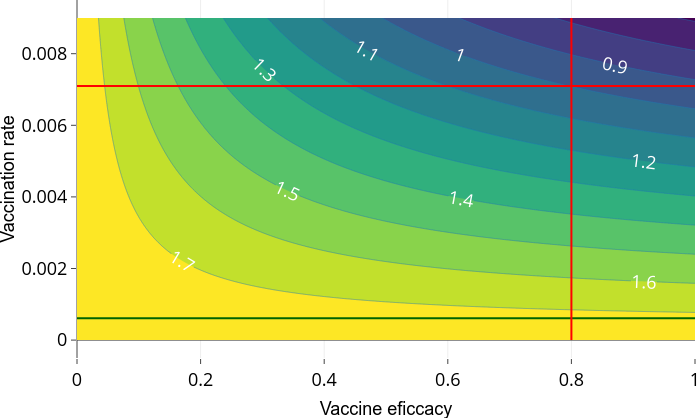
\includegraphics[scale=.50]{R0_contour.png}
    \caption{
        Contour plot  of $R_V$ like function of $\epsilon$ and
        $\lambda_V $ and with immunity average time by vaccination of half year.
        Blue line represents the value of $\lambda_{Vbase} = \num{0.000611}$,
        corresponding to a coverage $x_{coverage}=\num{0.2}$
        and a horizon time $T=\num{365}$. Purple lines show a scenario
        in which it is possible to reduce the $R_V$ value below one,
        considering a vaccine efficacy of $\epsilon =\num{0.8}$
        and a vaccination rate of $\lambda_V = num{0.7}$.
    }
    \label{R0_contour}
\end{figure}


    In the next section, the optimal control theory will be applied to propose
optimal vaccination dynamics that minimize the number of cases of symptomatic
infection and deaths due to the disease.
    \section{Optimal Vaccination
    policies}
        %!TEX root = main.tex


In the remains of this manuscript, we use the following definitions.
\begin{definition}[Constant vaccination policy]
Consider the model in \Cref{model1,eqn:model1_counters}. A constant 
    vaccination policy (CP) is a policy where the vaccination rate 
    $\psi_V$ remains constant for all time $t \in [0, T]$. 
    Thus the number of administered vaccine doses at time $t$
    with this CP results 
\begin{equation}
        \label{eqn:constant_policy}
        \psi_V \left(
            S(t) + E(t) + I_A(t) + R(t)
        \right) N.
    \end{equation}
\end{definition}

    Our main idea is taking $\psi_V$ as  \Cref{eqn:lambda_base}
and modulating it additively by a time function $u_V(t)$. 
We impose that 
$
    u_V(t)\in [-m_1 \psi_V, m_2 
    \psi_V],\forall t\in [0, T]
$,
 $m_1 \in [0,1]$, $m_2 \in \mathbb{Q}^{+}$, then term
\begin{equation}
    \label{eqn:vaccine_rate_modulation}
    \psi_V + u_V(t),
\end{equation}
amplifies or attenuates the constant vaccination rate $\psi_V$.
If $m_1 \in (0,1]$, then control signal $u_V(t)$ attenuates the vaccination 
rate $\psi_V$. Meanwhile, if $m_2 > 0$, then control signal $u_V(t)$ 
amplifies this vaccination rate.

We modify components equations corresponding to $S$, $V$, $X$ in 
\Cref{model1,eqn:model1_counters} by
\begin{equation}
    \label{eqn:counter}
    \begin{aligned}
        S'(t)  = &
            \mu \widehat{N} - f_{\lambda}S - 
            \left(
                \mu + (\psi_V + u_V(t)
            \right) S
        \\
            &
             + \omega_V V + \sigma_{R} R
        \\
        V'(t) = &
            \left(\psi_V + u_V(t)\right) S-(1-\varepsilon_V)
            f_{\lambda}V
        \\
            &-
             (\mu+\omega_V) V
        \\
        X'(t) =&
        \left(\psi_V + u_V(t)\right) (S + E + I_A + R).
    \end{aligned}
\end{equation}
%
Then our controlled dynamics reads
%
\begin{equation}
    \label{eqn:controlled_ode}
    \begin{aligned}
        S'(t)
        &=
        \mu \widehat{N} - f_{\lambda} S - 
        ( \mu + \psi_V +  u_V(t)) S + \omega_V V + \sigma_{R} R  
        \\
        E'(t)
        &=
        f_{\lambda} (S + (1-\varepsilon_V) V)
        - (\mu+\sigma_E) E
        \\
        I'_S(t)
        &=p
        \sigma_E
        E-(\mu + \alpha_S) I_S
        \\
        I'_A(t)
        &= (1 - p) \sigma_E E-(\mu + \alpha_A) I_A
        \\
        R'(t)
        &= (1 - \theta) \alpha_S I_S + \alpha_A I_A
        - (\mu + \sigma_{R}) R
        \\
        D'(t)&=
        \theta \alpha_S I_S
        \\
        V'(t)&=
        (\psi_V + u_V(t)) S -
        \left(
        (1 -\varepsilon_V) f_{\lambda} V +
        \mu + \omega_V
        \right) V
        \\
        X'(t)&=
        (\psi_V + u_V(t))(S + E + I_A + R)
        \\
        Y'_{I_S}(t) &=p
        \sigma_E E,
        \\
        \\
        S(0) &= S_0, \ E(0) = E_0, \ I_S(0) = I_{S_{0}},
        \\
        I_A(0) &= I_{A_{0}}, \ R(0) = R_0, \ D(0) = D_0,
        \\
        V(0) &= 0, \ X(0) = 0, \ Y_S(0) = Y_{S_0}
        \\
        \widehat{N}(t) &= S + E + I_S + I_A + R + V.
    \end{aligned}
\end{equation}

Formally we define a controlled vaccination policy as follows.

\begin{definition}[Controlled vaccination policy]
    Conforming the model in \Cref{eqn:controlled_ode} we say that
    $$
        \psi_V + u_V(t), \quad t \in [0, T],
    $$
    is a controlled vaccination policy (CVP). Then,
    $$
        (\psi_V + u_V (t))
        \left(
            S(t) + E(t) + I_A(t) + R(t)
        \right) N,
    $$
    denote the number of doses at time $t$ according to 
    the modulated vaccination rate $(\psi_V + u_V (t))$.
\end{definition}

    We aim to obtain time-control functions $u_V(\cdot)$ that hold natural 
modeling constraints\textemdash as a fixed bound for hospitalized 
prevalence and coverage at the final time\textemdash and optimize a 
conveniently cost functional. To this end, we have to assure our optimal controlled model solution, so we consider the functional space
\begin{equation}
    \label{eqn:picewise_continuous}
    \begin{aligned}
        \mathcal{U}[0,T] := &
        \left\{
            u_V: [0, T] \to \mathbb{R},
        \right.
            \\
            &
            \text{ such that $u_V(\cdot)$ bounded and}
            \\
            &
        \left.
            \text{ piecewise continuous}
        \right \}.
    \end{aligned}
\end{equation}

    Let ${x(t):= (S,E,I_S,I_A,R,D,V,X,Y_{I_S})^{\top}(t)}$
and control signal $u_V(\cdot)\in \mathcal{U}[0, T]$.
Following the guidelines of WHO-SAGE modeling questions \cite{sage2020},
we quantify the burden of COVID-19, according to the Disability-Adjusted Life 
Year (DALY) indicator. Adapting DALY's definition reported in 
\cite{WhoDALY}, we optimize the number of years of life lost with a 
controlled  vaccination policy. Our formulation 
calculates a minimum of the penalization functional 
%
\begin{align}
    \label{eqn:cost_functional}
    J(u_V) =
    a_D ( D(T) - D(0)) +
    a_S (Y_{I_S}(T) - Y_{I_S}(0)).
\end{align}
Here, $a_S$ and $a_D$ are parameters related to the definition of the Years of 
Life Lost (YLL) due to premature mortality and the Years Lost due to 
Disability (YLD). We estimate $a_D$ as the average remaining 
life expectancy at the age of
death, and according to the union of Mexico-City and Mexico-State data,
we set  $a_D = \SI{7.5}{years}$. Parameter $a_S$ is the product of a disability
weight (DW) and the average duration of cases until remission or death in years, that is,
$
a_S = DW \times \alpha_S^{-1}
$.
Here we postulate the disability weight as the arithmetic average of
disability weight regarding comorbidities reported in \cite{Jo2020}. Our
simulations employ $a_S= \SI{0.008418473}{years}$.
%
Thus, functional $J$ penalizes the pandemic burden\textemdash in Years
of Life Lost\textemdash due to mortality or disability. 

To describe vaccination coverage, we ask the terminal conditon
\begin{equation}
    \label{eqn:coverage_constrain}
    \begin{aligned}
     \varphi(x(T))&=X(T),
        \\
        S(T) &+ E(T) + I_S(T) + I_A(T) + R(T) + V(T) + D(T) = 1,
        \\
        X(T)
        &= x_{cover age},
        \\
        x_{coverage}
        & \in
        \left \{
        \text{Low(0.2)},\text{Mid(0.5)}
        \right \} .
    \end{aligned}
\end{equation}
That is, given the time horizon $T$, we set the vaccination coverage to 
\SI{20}{\percent} or \SI{50}{\percent} of the total population, and the rest 
of final states free. Likewise, we impose the path constraint
\begin{equation}
    \label{eqn:path_constrain}
    \Phi(x,t):= \kappa I_S(t) \leq B,
    \qquad \forall t \in [0, T],
\end{equation}
to ensure that critical symptomatic cases
will not overload healthcare services. Here $\kappa$
denotes hospitalization rate, and $B$ is the load capacity of the
health system. 

\begin{definition}[Admissible control vaccination policy]
    \label{dfn:admisible_policy}
    Let $(x(\cdot), u_V(\cdot))$ be a pair satisfying the ODE
    \eqref{eqn:controlled_ode}. Consider $\mathcal{U}[0, T]$
    as in \eqref{eqn:picewise_continuous}. If
    \begin{enumerate}[({\textbf{AC}}-1)]
        \item
            $u_V(\cdot) \in \mathcal{U} [0, T]$
        \item
            $u(t)\in [-m_1 \psi_V, m_2 \lambda_{V}],\ \forall t\in [0, T]$,
            \ $m_i \in \mathbb{Q}$
        \item
            $
            x(T) = (\cdot, \cdot, \cdot, 
                    \cdot, \cdot, \cdot,  
                    \cdot,  x_{coverage}, \cdot)^{\top}
            $
        \item
            $
                \kappa I_S(t) \leq B, \quad \forall t \in [0, T]
            $
    \end{enumerate}
    holds, then the CVP $\psi_V + u_V (\cdot)$ is
    admissible.
\end{definition}
In other words, an admissible vaccination policy (AVP) is a CVP that 
satisfies the coverage and hospitalization constraints imposed on
model \eqref{eqn:controlled_ode}. Furhter,
if an AVP optimizes functional cost \eqref{eqn:cost_functional}, then this AVP is an optimal vaccination policy (OVP). Formally we have the following definition.
\begin{definition}[Optimal Vaccination Policy]
    Let $(x(\cdot), u_V(\cdot))$ a pair that satisfies the ODE 
    \eqref{eqn:controlled_ode} such that (\textbf{AC}-1)--(\textbf{AC}-4) of 
    \Cref{dfn:admisible_policy} holds. Let cost functional $J$ as in 
    \eqref{eqn:cost_functional}. If
    \begin{equation}
        \begin{aligned}
            J(u_V) &=
                \min_{u  \in \mathcal{U}^{\star}}
                     J(u),
            \\
            \mathcal{U}^{\star} &: =
                \mathcal{U}[0, T]
                \cap\{
                    u(\cdot): \text{(ADC-1)--(ADC--4) holds}
                \},
        \end{aligned}
    \end{equation}
    then  $\psi_V + u_V(\cdot)$ is an optimal vaccination policy.
\end{definition}
\begin{rmk}
    Optimal vaccination amplifies or attenuates the estimated
    baseline $\psi_V$ in an interval $[\psi_V^{\min}, \psi_V^{\max}]$
    to optimize functional $J(\cdot)$\textemdash minimizing  symptomatic incidence and death reported cases in DALYs and satisfying hospitalization occupancy and coverage constraints.
\end{rmk}
    
    We aim to minimize the cost functional
\eqref{eqn:cost_functional}\textemdash over an appropriated
space\textemdash subject to the dynamics in \Cref{eqn:controlled_ode},
coverage related to the boundary condition \eqref{eqn:coverage_constrain}, 
and path constraints \eqref{eqn:path_constrain}. We call this kind of 
policies as optimal vaccination policies (OVP). That is, we seek 
vaccination policies that solve the following problem.

\emph{Optimal Control Problem (OCP):}
    Find the optimal vaccination rate $(\psi_V + u_V^{*})$ such that, 
    
\begin{equation}
    \label{eqn:optimal_control_problem}
    \begin{aligned}
        J(u_V^*) &=
            \min_{u_V  \in \mathcal{U}^{\star}}
        J(u_V) 
        \\
        J(u_V) &:=
        a_D ( D(T) - D(0)) +
        a_S (Y_{I_S}(T) - Y_{I_S}(0))
        \\
        \text{subject to} &
        \\
        f_{\lambda}
        & :=
        \frac{\beta_S I_S + \beta_AI_A}{\widehat{N}}
        \\
        S'(t)
        &=
        \mu \widehat{N}-f_{\lambda} S -( \mu + \psi_V +  u_V(t)) S+ \omega_V V + \sigma_{R} R
        \\
        E'(t)
        &=
        f_{\lambda} (S + (1-\varepsilon_V) V)
        - (\mu+\sigma_E) E
        \\
        I'_S(t)
        &=p
        \sigma_E
        E-(\mu + \alpha_S) I_S
        \\
        I'_A(t)
        &= (1 - p) \sigma_E E-(\mu + \alpha_A) I_A
        \\
        R'(t)
        &= (1 - \theta) \alpha_S I_S + \alpha_A I_A
        - (\mu + \sigma_{R}) R
        \\
        D'(t)&=
        \theta \alpha_S I_S
        \\
        V'(t)&=
        (\psi_V + u_V(t)) S -
        \left(
        (1 -\varepsilon_V) f_{\lambda} V +
        \mu + \omega_V
        \right) V
        \\
        X'(t)&=
        (\psi_V + u_V(t))(S + E + I_A + R)
        \\
        Y'_{I_S}(t) &=p
        \sigma_E E,
        \\
        \\
        S(0) &= S_0, \ E(0) = E_0, \ I_S(0) = I_{S_{0}},
        \\
        I_A(0) &= I_{A_{0}}, \ R(0) = R_0, \ D(0) = D_0,
        \\
        V(0) &= 0, \ X(0) = 0, \ Y_S(0) = Y_{S_0}, 
        \ X(T) = x_{coverage},
        \\
        u_V(\cdot) & \in [u_{\min}, u^{\max}],
        \\
        \kappa I_S(t) & \leq B, \quad \forall t \in [0, T],
        \\
        \widehat{N}(t) &= S + E + I_S + I_A + R + V.
    \end{aligned}
\end{equation}
%
\Cref{Fig:SchemeModel_opt} 
illustrates the main ideas of the above discussion.
\Cref{tbl:ocp_parameters_description} 
enclose parameter information of the functional cost and constraints. 

Existence of solution to our (OCP) in \Cref{eqn:optimal_control_problem} drops
in the theory developed by Francis Clark
\cite[see e.g.][Thm. 23.11]{Clarke2013}. Since we aim to simulate
hypothetical scenarios, we omit here a rigorous proof. Instead, we refer
interested readers to \cite{Sethi1995,Lenhart2007} and the reference therein.
%
\begin{figure*}[tbh]
    \centering
    \includegraphics[scale = 1]{Figure_5.pdf}
    \caption{Compartmental diagram of COVID-19 transmission dynamics
        that
        includes optimal vaccination dynamics, penalization and a path
        constraint.}
    \label{Fig:SchemeModel_opt}
\end{figure*}
%
\begin{table*}[htb]
    \centering
    \begin{tabular}{%
            >{\centering}
            p{0.1\textwidth}
            p{0.38\textwidth}
            p{0.15\textwidth}
            p{0.15\textwidth}
        }
        \toprule
        \textbf{Symbol}
        & \textbf{Description}
        & \textbf{Value}
        & \textbf{Ref}
        \\
        \midrule
        $a_D$
        &
        Penalization weight due to  premature mortality (YLL)
        and estimated from Mexico-City an Mexico-State data
        & $\SI{7.5}{years}$ & \cite{WhoDALY,DataMX}
        \\
        $a_S$
        &
        Penalization weight due to disability (YLD)
        & $\SI{0.008418473}{years}$ & \cite{Jo2020}
        \\
        $x_{coverage}$
        &
        Covering constraint at time horizon $T$
        & & \cite{sage2020}
        \\
        $\kappa$
        &
        Hospitalization rate
        &
        \num{0.05}
        &
        Estimated
        \\
        $B$
        &
        Health service capacity in number of beds
        &
        \num{9500}
        &
        Estimated
        \\
        \bottomrule
    \end{tabular}
    \caption{
        Parameters regarding the
constraints conditions and cost functional of the OCP
\eqref{eqn:optimal_control_problem}.}
    \label{tbl:ocp_parameters_description}
\end{table*}
    \section{Numerical experiments}
        %!TEX root = main.tex
\subsection{Methodology}
        We apply the so-called transcript method to solve our (OCP).
    This method transforms the underlying problem of
    optimizing functional governed by a differential equation into a
    finite-dimensional optimization problem with restrictions. To fix ideas,
    let $x$, $u$ respectively denote state and control, and consider the
    optimal control problem
    \begin{equation*}
        \begin{aligned}
                & \min J(x(\cdot), u(\cdot)) = g_0(T, x(T))
                & \text{Functional cost}
            \\
                & \dot{x} = f(t, x(t), u(t)),
                \quad\forall t \in [0, T],
                & \text{Dynamics}
            \\
                & u(t) \in \mathcal{U}[0, T] \text{for a.e. } t\in [0, T]
                & \text{Admissible controls}
            \\
                & g(x(t), u(t)) \leq 0
                & \text{Path constrain}
            \\
                & \Phi(x(0), x(T)) = 0
                & \text{Boundary conditions}.
        \end{aligned}
    \end{equation*}
        Then, transcription methods transform this infinite-dimensional
    optimization problem into a finite dimension problem (NLP) via
    discretization of dynamics, state, and control.  For example, if we
    employ the Euler method with a discretization of $N$ constant steps with
    size $h$, then we can solve
        \begin{equation}
            \label{eqn:nlp}
            \begin{aligned}
                    &\min g_0(t_N, x_N)
                \\
                    &
                        x_{i+1} = x_i + h f(x_i, u_i),
                    & i = 0, \dots, N - 1
                \\
                    &
                        u_i \in \mathcal{U},
                    & i = 0, \dots, N
                \\
                    &
                        g(x_i, u_i) \leq 0,
                    & i = 0, \dots, N
                \\
                    &
                    \Phi(x_0, x_N) = 0,
                    &i = 0, \dots, N,
            \end{aligned}
        \end{equation}
    where $x_i \approx x(t_i)$,
    $u_i \approx u(t_i)$ in the grid
    $$
        \left\{
            t_0 = 0,\quad
            t_i = i h \ (i=1,\dots, N-1),\quad
            t_N = T
        \right\}.
    $$
    Let $Y = \{x_0, \dots, x_N, u_0,\dots u_N\}$.
    Thus \Cref{eqn:nlp} defines a nonlinear programming problem on the
    discretized state and control variables of the form
    \begin{equation}
        \label{eqn:nlp_form}
        \begin{aligned}
            &
            \min F(Y)
        \\
        \text{such that} &
        \\
            &
            LB \leq C(Y) \leq UB .
        \end{aligned}
        %\tag{NLP}
    \end{equation}
    %
        The numerical analysis and design of transcript methods is a well
    established  and active research numerical field. There is a vast
    literature about robust methods and recently, implementations have been
    developed in vogue languages like Julia
    \cite{DunningHuchetteLubin2017, LubinDunningIJOC}, Python \cite{libcmaes},
    Matlab \cite{matlabOpt}, and others. We refer the reader to
    \cite{Betts2001,Seywald1993} for a more systematic discussion.

        Our simulations rely on the \verb|Bocop| package
    \cite{Bocop,BocopExamples} to solve our (OCP). Bocop is part of the
    development of the INRIA-Saclay initiative for open source optimal control
    toolbox and supported by the team Commands. BOCOP solves the NLP problem in
    \Cref{eqn:nlp_form} by the well known software \textsc{Ipopt} and using
    sparse exact derivatives computed by ADOL-C.

        We provide in \cite{gitHub} a GitHub repository with all regarding R
    and Bocop sources. This repository also encloses data sources and python
    code to reproduce all reported figures.

\subsection{Simulation of hypothetical scenarios}
        We follow the guidelines reported by the WHO Strategic Advisory Group
    of Experts (SAGE) on Immunization Working Group on COVID-19 Vaccines
    modeling questions presented in \cite{sage2020}. According to this SAGE's
    document, we simulate scenarios to illustrate vaccination policies'
    response with a preventive vaccine. We aim to contrast the impact of the
    burden of COVID-19 mitigation regarding
    \begin{enumerate}[(\textbf{SCN}-1)]
        \item Optimal versus constant vaccination policies
        \item Vaccine efficacy
        \item Induced vaccine immunity
        \item Natural immunity
    \end{enumerate}

    \added[id=SDIV, comment = cites]{
        We consider vaccine profiles\textemdash efficacy and induced vaccine
    immunity\textemdash compatible with  the firms Pfizer-BioNTech,
    Moderna, Astra-Zeneca, Gamaleya Research Institute
    Johnson \& Johnson, Sinovac Biotech among others.
    Further, since reinfection and induced vaccine immunity parameters remain
    unavailable, we see pertinent to explore the effect of plausible settings.
    }
%
    \begin{rmk}
        Optimal vaccination policy implies that number of doses per unit time
        described by

        $$
            (\psi_{V}+u_V(t))(S(t)+E(t)+I_A(t)+R(t))
        $$
        mitigates the outbreak in optimal form, where optimal is defined in
        terms of function $J$ (see \Cref{eqn:cost_functional}), that is
        minimizing years of life lost in DALYs.
        Counterfactual scenarios implies $u_V(t)=0$. Without vaccination
        scenarios we means $\psi_{V} + u_V(t)=0,  \ \forall t \in [0, T]$.
    \end{rmk}
%
    \begin{rmk}
        We assume positive prevalence of all epidemiological
        classes according to the following hypothesis:
        \begin{enumerate}[{(IC)}-1]
            \item
                The implemented initial conditions for our
                numerical experiments are
                hypothetical and not reflects the
                actual data reported by Mexico-City and Mexico-State
                health authorities. The initial conditions are taken such
                that an outbreak is on its growth phase
                (see \Cref{Fig:initial_conditions}).
            \item
                We suppose that around of \SI{30}{\percent}
                of the population is under Lockdown and is
                enclosed along with recovered class $R$. That
                is, $R(0)$ encircle mainly  children, senior,
                home office, people with low mobility and
                COVID-19 recovered individuals.
            \item
                Our numerical results are of
                qualitative nature and non necessarily sustain
                forecasting or follows the actual profile of the
                underlying COVID-19 pandemic data.
        \end{enumerate}
    \end{rmk}

    \begin{figure*}[h!]
        \centering
        \includegraphics[scale=1]{Figure_6.png%Figure_23.pdf
        }
        \caption{
            Hypothetical scenario when considering COVID-19 transmission
            dynamics without vaccination process. Blue line shows symptomatic
            prevalence dynamics. Red cross represents the initial date of
            simulations.
        }
        \label{Fig:initial_conditions}
    \end{figure*}

    \Cref{tbl:scene_parameters} encloses a brief description
    and parameter values regarding each scenario. The reader
    can also access the web
    \verb|Chart Studio Graph| of each figure regarding data and
    \verb|plotly| \cite{plotly} visual representation.
%
    \begin{table*}[tbh]
        \centering
        \begin{tabular}{%
                >{\centering}
                p{0.1\textwidth}
                p{0.23\textwidth}
                p{0.57\textwidth}
            }
            \toprule
            \textbf{Simulation Scene}
            & \textbf{\qquad Description}
            & \textbf{Set-up} \quad
            $(x_{coverage}, T, \varepsilon_{V}, \omega_{V}^{-1}, \sigma_{R}^{-1})$
            \\
            \midrule
            \textbf{(SCN-1)}
            &
            Likening between optimal and constant
            vaccination policies.
            &
            (%
            \SI{20}{\percent},
            \SI{180}{days},
            \SI{70}{\percent},
            \SI{730}{days},
            \text{lifelong}
            )
            \\
            \textbf{(SCN-2)}
            &
            Vaccine efficacy blow
            &
            (%
            \SI{50}{\percent}, %
            \SI{365}{days}, %
            $\left\{
            \SI{50}{\percent},
            \SI{70}{\percent},
            \SI{90}{\percent}
            \right\}
            $, %
            \SI{730}{days}, %
            \SI{180}{days}
            )
            \\
            \textbf{(SCN-3)}
            &
            Induced vaccine immunity period
            &
            (%
            \SI{50}{\percent}, %
            \SI{365}{days}, %
            \SI{90}{\percent},
            $\left\{
            \SI{180}{days},
            \SI{365}{days},
            \SI{730}{days}
            \right\}
            $, %
            \SI{365}{days}%
            )
            \\
            \textbf{(SCN-4)}
            &
            Natural immunity period
            &
            (%
            \SI{50}{\percent}, %
            \SI{365}{days}, %
            \SI{90}{\percent}, %
            \SI{730}{days}, %
            $
            \left\{
                \SI{90}{days},
                \SI{180}{days},
                \SI{365}{days}
            \right\}
            $%
            )
            \\
            \bottomrule
        \end{tabular}
        \caption{
            Setup parameters for counterfactual and response scenarios. See
            \Cref{tbl:fixed_parameters} for the rest of parameters.}
        \label{tbl:scene_parameters}
    \end{table*}
%

    To perform the simulations corresponding to the scenarios presented in
\Cref{tbl:scene_parameters}, we fix the parameter values as in
\Cref{tbl:fixed_parameters-OCM}.
%
\begin{table*}[tbh]
    \begin{center}
        \begin{tabular}{rc@{}c}
            \toprule
            \multicolumn{3}{c}{\textbf{Parameters values}}
            \\
            \midrule
            \\
                & \multicolumn{2}{c}{\textbf{(SCN-1)--(SCN4)}}
                \\
                \cmidrule{2-3}
                \\
                $\beta_S$, $\beta_A$, $\alpha_{S}$, $\alpha_{A}$, $\sigma_{E}$,
                $\mu$, $\theta$, $p$
                & \multicolumn{2}{c}{\Cref{tbl:fixed_parameters}}
            \\
                $a_D$, $a_S$, $\kappa$, $B$
                & \multicolumn{2}{c}{\Cref{tbl:ocp_parameters_description}}
            \\

            \\
                & \textbf{(SCN-1)}
                & \textbf{(SCN-2)}--\textbf{(SCN-4)}
            \\
                \cmidrule{2-3}
                %\cmidrule{3-3}
            %\\
%                \cmidrule{3-3}
%            \\
            $\psi_{V}$
                & \num{0.00123969}
                & \num{0.00189903}
            \\
                $u_{min}$
                & \num{-0.000619845}
                & \num{-0.00094952}
            \\
                $u_{max}$
                & \num{0.00619845}
                & \num{0.00474758}
            \\
            \bottomrule
        \end{tabular}
        \caption{%
            Fixed parameters values of system in
            \Cref{eqn:optimal_control_problem}.}
        \label{tbl:fixed_parameters-OCM}
    \end{center}
\end{table*}
%
\section*{Optimal Versus Constant Vaccination Policies: (SCN-1)}
        To fix ideas, we display in
        \Cref{fig:lifelongvaccinationpolicies,%
        fig:lifelongvaccinationpoliciesOutbreak}
    the counterfactual scenario regarding no intervention. We
    contrast a constant vaccination policy (CP) and optimal vaccination
    policy (OP) with a vaccine profile of efficacy
    $\varepsilon_V = \SI{70}{\percent}$, vaccine-induced immunity
    $\omega_V^{-1} = \SI{730}{days}$ and a campaign for \SI{20}{\percent}
    of coverage at \SI{180}{days}. \Cref{fig:lifelongvaccinationpolicies}
    suggests that the OP improves CP vaccination policy response according to
    the disease burden due to mortality, and morbidity.
    \Cref{fig:lifelongvaccinationpoliciesOutbreak} confirms this improvement by
    comparing disease dynamics with and without vaccination. We observe CP and
    OP reduce disease levels. Although both campaigns administrate the same
    number of vaccine doses, OP vaccination implies fewer deaths and
    symptomatic cases.
    \deleted[id=SDIV, comment= Fix this paragraph]{Figure 3 %
        %\Cref{fig:lifelongvaccinationpolicies}
    shows a scenario whit
    $R_0>1$. The underlying vaccine reproductive number $R_V$
    remains below to $R_0$. This Figure illustrates the strong relation between disease mitigation, vaccine efficacy $(\varepsilon_{V})$,
    and vaccination rate $(\psi_{V})$. Further, given a dynamic
    without vaccine intervention and $R_0>1$, $R_V$ projects a
    minimal vaccination rate to drive this dynamic to the disease-free state
    but subject to vaccines with particular efficacy.}
    %
    \begin{figure*}[tbh!]
        \centering
        \includegraphics[scale=1]{Figure_7.png}
        \caption[Effect of the vaccination policy on the burden COVID-19]{%
        Effect of the vaccination policy on the burden COVID-19 for a 20\%
        coverage at time horizon of half year.
        (A) Vaccination policies' response regarding constant ($\psi_V$)
        and optimal ($\psi_V+u_V(t)$)  vaccination rates in the burden of
        COVID-19 quantified in DALYs. (B) Evolution of the
        vaccination covering according to each policy.
        (C) Vaccination schedule for each vaccination policy.
        Blue translucent color corresponds to policies with constant
        vaccination rate \num{0.00123969}. Green tone is related to the
        optimal vaccination policy. For counterfactual reference (panel A),
        black line-gray shade represents the burden of COVID-19 without
        vaccination.
        See \href{https://plotly.com/~MAAZ/366/}{%
                https://plotly.com/~MAAZ/366/}
        for plotly visualization and data.
        }
        \label{fig:lifelongvaccinationpolicies}
    \end{figure*}
    \begin{figure*}[tbh!]
        \centering
        \includegraphics[scale=1]{Figure_8.png}
        \caption[Effect of the vaccination policy on outbreak evolution.]{
        Effect of the vaccination policy on outbreak evolution.
        (A) Optimal vaccination policy reaches a better response in mitigating
        symptomatic cases than a policy with a constant vaccination rate.
        (B) Gray and blue shaded translucent regions denote the number of
        saved lives per \SI{100000}{inhabitants}.
        The optimal vaccination rate (grey-blue) improves the number of saved
        lives per \SI{100000}{inhabitants} of the constant rate $\psi_V$.
        Data and web visualization in
        \href{%
            https://plotly.com/~MAAZ/370/
        }{https://plotly.com/~MAAZ/370/}.
        }
        \label{fig:lifelongvaccinationpoliciesOutbreak}
    \end{figure*}
%
    \section*{Vaccine Efficacy (SCN-2)}
        \comment[id=SDIV]{Fix.
            Say that has been approved developments in
            Mexico
        }
        In February 2021, multiple vaccines have been rolled out to prevent
        COVID-19 disease. \Cref{tbl:vaccine-efficacy-portfolio} contains
        information on developments that we consider relevant to explore a wide
        range of plausible vaccine-efficacies.
        \begin{table}[htb]
            \centering
            \begin{tabular}{%
                p{3cm}
                p{2cm}
                p{3.5cm}
                P{2cm}
            }
            \toprule
            \textbf{Developer} &
            \textbf{Vaccine Name} &
            \textbf{Vaccine Efficacy \%, (95\% CI)} &
            %\textbf{Status} &
            \textbf{Reference}
                \\
                 \midrule
                \\
                    Pfizer-BioNTech
                        & BNT162b2
                        & \num{95} (\num{90.3}–\num{97.6})
                        %& Approved for emergency use in the USA, Mexico,
                        % Germany, UK, and other countries
                        & \cite{vaccine_tracker2020}
                \\
                    Gamaleya Institute
                        & Sputnik V
                        & \num{91.6} (\num{85.6}–\num{95.2})
                        %& Early use in Russia. Emergency use Mexico an other
                        %countries.
                        & \cite{Logunov2021}
                \\
                    Oxford University-AztraZeneca
                        & AZD1222
                        & \num{74.6} (\num{41.6}-\num{88.9})
                        %& Approved for emergency use in the USA, Mexico,
                        & \cite{Emary2021}
                \\
                    Johnson \& Johnson
                        & Ad26.COV2.S
                        & \SI{72}{\percent}
                        %& Approved for emergency use in the USA, Mexico,
                        & \cite{johnsonandjohnson}
                \\
                    Sinovac Biotech
                        & CoronaVac
                        & 50.4\%
                       % & Approved in China. Emergency use in Brazil, other
                       % countries.
                        &\cite{vaccine_tracker2020}
                \\
            \bottomrule
            \end{tabular}
            \caption{Vaccine efficacy of some
            to the platforms approved to emergency use.}
            \label{tbl:vaccine-efficacy-portfolio}
        \end{table}
%
    \begin{itemize}
        \item
            by Pfizer-BioNTec has
            95\% effectiveness (95\% CI, 90.3 to 97.6) \cite{Polack2020};
        \item
            Sputnik V by Gamaleya has
            91.6\% effectiveness (95\% CI 85.6–95.2) \cite{Logunov2021};
        \item
            AZD1222 by Oxford-48AstraZeneca has vaccine efficacy for
            different virus lineages with 74.6\% [95\% CI 41.6-88.9] and
            84 \% [95\% CI 70.7-91.4], respectively \cite{Emary2021};
        \item
            Ad26.COV2.S by Johnson \& Johnson has a vaccine's efficacy against
            moderate and severe disease ranged from one country to another:
            72\% in the US, 66\% in Latin America and 57\% in South Africa
            \cite{johnsonandjohnson};
        \item CoronaVac by Sinovac Biotech has 50.4\% effectiveness
            \cite{vaccine_tracker2020}.
    \end{itemize}

    \Cref{fig:efficiencyvaccineprofile,fig:efficiencyvaccineprofileOutbreak}
    display the optimal vaccination policy's response  according to three
    vaccines with different efficacy. \Cref{fig:efficiencyvaccineprofile}A
    displays COVID-19 burden in DALYs for policies with
    \SI{50}{\percent},
    \SI{70}{\percent},
    \SI{90}{\percent}
    vaccine-efficacies.
    Figures \ref{fig:efficiencyvaccineprofile}B-C also illustrate the effect
    of vaccine-efficacies on coverage and optimal vaccination policy
    respectively.
    \added[id=SDIV, comment={how?, be concise}]{
    We observe that vaccine-efficacy influences design optimal policy.}
    According to \SI{50}{\percent} coverage at a time horizon of
    \SI{1}{year}, \Cref{fig:efficiencyvaccineprofileOutbreak} displays an
    improvement of at least three times in the prevalence of symptomatic cases
    and saved lives concerning the uncontrolled
    outbreak. \Cref{fig:efficiencyvaccineprofileOutbreak} reflects this
    effect in the mitigation
    symptomatic prevalence (A) and
    the number of saved lives (B) shaded by the translucent
    grey (50\% vaccine efficacy), grey-blue (70\% vaccine efficacy), and
    grey-blue-red (90\% vaccine efficacy).
%
%------------------------------------------------------------------------------
% Vaccine efficacy gradient
%
    \begin{figure*}[htb]
        \centering
        \includegraphics[scale=1]{%
            Figure_9.png%./EfficiencyVaccineProfile_v2.png%
        }
        \caption[The response of COVID-19 to vaccine efficacy]{
            The response of COVID-19 burden to vaccine efficacy.
            (A) COVID-19 burden response quantified in DALYs per \SI{100000}{
            inhabitants}  to vaccines with efficacy of
            \SI{50}{\percent} (blue),
            \SI{70}{\percent} (red) and \SI{90}{\percent}(green).
            (B) Coverage evolution to reach \SI{50}{\percent} of the total
            population vaccinated.
            (C) Optimal vaccination doses schedule according to the
            different efficacies. See
            \href{https://plotly.com/~MAAZ/358/}{%
                https://plotly.com/~MAAZ/358/} for
            visualization and data.
        }
        \label{fig:efficiencyvaccineprofile}
    \end{figure*}
%
    \begin{figure*}[htb]
        \centering
        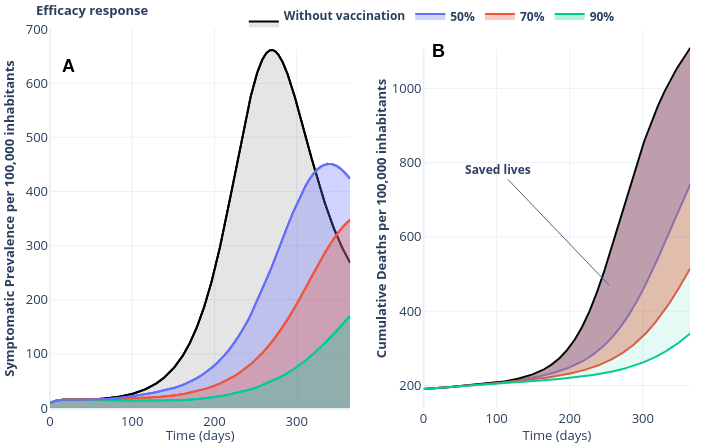
\includegraphics[scale=1]{%
            Figure_10.png%./EfficiencyVaccineProfileOutbreak.png%
        }
        \caption[The effect of vaccine efficacy over
            COVID-19 symptomatic prevalence and morbidity]{
            The effect of vaccine efficacy over COVID-19 symptomatic
            prevalence and morbidity.
            (A) Effect of vaccine-efficacy of
            \SI{50}{\percent} (blue), \SI{70}{\percent} (red)
             and \SI{90}{\percent} (green) on prevalence
             of symptomatic cases per \SI{100000}{inhabitants}.
            (B) Effect of vaccine-efficacy on the number of saved lives.
            See
            \href{https://plotly.com/~MAAZ/375/%
            }{https://plotly.com/~MAAZ/375/} for data and
            visualization.
        }
        \label{fig:efficiencyvaccineprofileOutbreak}
    \end{figure*}

\section*{Vaccine-induced immunity (SCN-3)}
    Vaccine response also is strongly related to its induced immunity
    \textemdash parameter that remains poorly understood
    \cite{Jeyanathan2020}.
    Here, we contrast two vaccines with different induced-immunity. Let
    denote by $vax_1$, $vax_2$, $vax_3$ vaccines with an induced-immunity
    capacity of a half, one, and two years, respectively, and common efficacy
    of \SI{90}{\percent}.
    Consider a vaccine camping of time horizon of one year and
    \SI{50}{\percent} coverage. Taking the same dynamics parameters, that is
    initial conditions, and baseline parameters, as in
    \Cref{tbl:fixed_parameters}, we explore a counterfactual scenario with an
    uncontrolled outbreak of $R_0 = \num{1.79493}$ and three controlled
    dynamics according to vaccines $vax_1$, $vax_2$, $vax_3$. Thus, according
    to these immunity parameters and factor defined in
    \Cref{eqn:mitigation_factor}, respectively, results
    $R_V^{[vax_1]} = \num{1.38555}$,
    $R_V^{[vax_2]} = \num{1.13913}$,
    $R_V^{[vax_3]} = \num{0.86756}$
    for vaccine immunities periods of a half, one, and two years. We display in
    \Cref{fig:induced_immunity_vaccine_profile} the response of the
    vaccines $vax_1$, $vax_2$ and $vax_3$. \az Since optimal vaccination
    policies are similar, \Cref{fig:induced_immunity_vaccine_profile} A
    suggests vaccine-induced immunity rate is not determinant in the
    vaccination schedule design. \st{Since in this  scenario set time
    horizon is of one year, the optimal policies follow similar schedules and
    imply similar gains in the number of years of life lost. Despite these
    similarities,} \za \Cref{fig:inducedimmunity_vaccine_outbreak}
    displays \az \st{in panel A dramatically gain respect to} a wide reduction
    of disease levels concerning the uncontrolled outbreak.
    \st{\textemdash since $R_V ^{[vax_2]}$ is near to one, prevalence
    fall-down more than five times and because $R_V ^{[vax_3]}$ is less that
    one, prevalence of symptomatic cases tends to zero with damped
    oscillations.
    Figure 13 also endorses this gain regarding
    saved lives (B). This gain is}
    It happens as a consequence of the vaccine reproduction number reductions.
    For this scenario, we observe that it is unnecessary to reduce $R_V$ below
     one to obtain notable mitigation. The disease level reduction
    represented by the shaded grey region (a half year),
    grey-green region (one years) and grey-green-red region (two years).
    \za
%
%-------------------------------------------------------------------------------
% Induced vaccine immunity gradient
    \begin{figure*}[htb]
        \centering
        \includegraphics[scale=1]{%
        Figure_11.png%InducedImmunityVaccineProfile%
        }
        \caption[
            Effect of Vaccine-induced immunity effect on the burden of COVID-19.
        ]{
            Effect of vaccine-induced immunity on the COVID-19 burden.
            (A) Effect on the burden of COVID-19 quantified in DALYs per
            \SI{100000}{inhabitants} due to vaccine-induced immunity of
            \SI{180}{days} (green), \SI{365}{days} (red) and 730 days (blue).
            (B) Coverage evolution to reach \SI{50}{\percent} of the total
            population vaccinated.
            (C) Optimal vaccination doses schedule according to the different
            vaccine-induced immunities. Visualization and data in
            \href{https://plotly.com/~MAAZ/407/}{%
                https://plotly.com/~MAAZ/407/
            }.
        }
        \label{fig:induced_immunity_vaccine_profile}
    \end{figure*}
    %
    \begin{figure*}[htb]
        \centering
        \includegraphics[scale=1]{Figure_12.png}
        \caption[Effect of vaccine-induced immunity
                on mitigation and saved lives of COVID-19 outbreak]{
            Effect of vaccine-induced immunity on mitigation and saved lives of COVID-19 outbreak.
            (A)  Effect of vaccine-induced immunity on mitigation of symptomatic prevalence per \SI{100000}{inhabitants}.
            (B) The number of saved lives. See
            \href{https://plotly.com/~MAAZ/416/}{%
                https://plotly.com/~MAAZ/416/}.
        }
        \label{fig:inducedimmunity_vaccine_outbreak}
    \end{figure*}
%------------------------------------------------------------------------------
\section*{Natural Immunity Hypothesis (SCN-4)}
%
     ``Reinfections raise questions about long-term immunity to
     COVID-19 and the prospects for a vaccine'',  reported
    Heidi Ledford in \cite{Ledford2020b}. Following this line, we
    display in \Cref{%
            fig:natural_recovering_profile,%
            fig:natural_recovering_outbreak}
    the vaccine's response with \SI{90}{\percent} efficacy and
    contrasting with  natural immunity periods of \SI{90}{days},
    \SI{180}{days}, and \SI{365}{days}. Here, the adjective ``natural''
    denotes the immunity that an individual develops after recovering from a
    previous bout of COVID-19 without vaccination.
    When implementing an optimal vaccination strategy, if natural
    immunity lasts one year, the burden of COVID-19 falls until around
    \SI{120}{DALYs}. We confirm this behavior in the prevalence of symptomatic
    cases and cumulative deaths, as displayed in
    \Cref{fig:natural_recovering_outbreak}. When natural immunity is
    \SI{365}{days}, the gain in mitigation concerning a natural immunity of
    \SI{90}{days} is at least \num{100} times, while the number of deaths
    with a natural immunity of \SI{90}{days} reach \num{845} cases per
    \SI{100000}{inhabitants}, in contrast, of \SI{206} when natural immunity is
    \SI{365}{days}. Thus, this simulation suggests that natural immunity
    plays a vital role in the controlled outbreak's behavior, which is
    consistent with the conclusions reported in \cite{Jeyanathan2020}.
%
    \begin{figure*}[tbh!]
        \centering
        \includegraphics[scale=1]{Figure_13.png}
        \caption[Effect of natural immunity on the burden of COVID-19]{
            Effect of natural immunity on the burden of COVID-19.
            (A) Effect on the burden of COVID-19 quantified in DALYs per
            100,000 inhabitants due to natural immunity of 90 days (red),
            180 days (blue) and 365 days (green).
            (B) Coverage evolution to reach \SI{50}{\percent} of the total
            population vaccinated.
            (C) Optimal vaccination doses schedule according to the different
            natural immunities. See
            \href{https://plotly.com/~MAAZ/402/}{%
                https://plotly.com/~MAAZ/402/}.
        }
        \label{fig:natural_recovering_profile}
    \end{figure*}
%
    \begin{figure*}[h!]
        \centering
        \includegraphics[scale=1]{Figure_14.png}
        \caption[Vaccine induced immunity profile.]{
            Effect of natural immunity on mitigation and saved lives of
            COVID-19 outbreak.
            (A) Effect of  immunity on mitigation of
            symptomatic prevalence per \SI{100000}{inhabitants}.
            (B) Number of saved lives. Plotly visualization and data in
            \href{https://plotly.com/~MAAZ/406/}{%
                https://plotly.com/~MAAZ/406/
            }.
        }
        \label{fig:natural_recovering_outbreak}
    \end{figure*}
    \section{Conclusions and Discussions}
        
At the date of writing this article, humankind lacks strategies to
eradicate COVID-19.  Although NPIs implemented in most countries prevent
citizens from being infected, these strategies leave them
susceptible\textemdash people can not develop immunity to face futures waves.
Thus, vaccination becomes the primary pharmaceutical measure to recover life's
style before the pandemic. However, this vaccine has to be effective and well
implemented in global
vaccination programs. Thus new challenges as its distribution, stocks,
politics, vaccination efforts, among others, emerge. A fair distribution and
application strategy is imperative to manage the available resources,
especially in developing countries.

%\paragraph{Statement of principal findings}
We established an optimal control problem to design vaccination strategies
where vaccination modulates dynamics susceptibility through an imperfect
vaccine. We aimed to provide vaccination policies that minimize the lost life
years due to disability or premature death by COVID-19, determined by
cumulative deaths and cumulative incidence. Policies' acts in the minimization
of infected people's prevalence and the number of deaths.

%\paragraph{Strengths and weaknesses of the study}
Our simulations suggest a better response with optimal vaccination policies
than policies with a constant vaccination rate. For example, the optimal policy
schedule in scenario \textbf{SCN-1} increases the number of doses in the
scheme's initial stage. This vaccination scheme improves the mitigation of the
symptomatic prevalence, the incidence of deaths, and in consequence, the years
of life lost quantified in DALYs.
%

Emerging press releases reported that Pfizer's, Russian Sputnik V,
and Moderna's coronavirus vaccines reach efficacy over \SI{90}{\percent}
\cite{cnn_health_2020,reuters2020, cnn_health_2020b}. However,
this information remains under development. Thus vaccine efficacy scenarios of
\SI{50}{\percent}, \SI{70}{\percent}, and \SI{90}{\percent} \textbf{(SCN-2)}
illustrate the effect on optimal vaccination policies' schedule by pointing
when to intensify the number of doses. According to the time horizon of one
year and coverage of 50\%, our numerical experiments suggest that
\SI{90}{\percent} vaccine efficacy reduces around three times the number of
deaths regarding the dynamics without vaccination. Likewise, these vaccines
reach a gain of eighteen times in the years of life lost compared to the
without vaccination scenario.


Our numerical experiments also illustrate vaccine-induced immunity's
relation between the reproductive vaccination number $R_V$ and vaccination
policies \textbf{(SCN-3)}. Considering an outbreak with a reproductive number
$R_0$ of \num{1.794 93}, vaccine-induced immunity of \num{365} or
\SI{730}{days} implies a reduction of $R_0$\textemdash dropping its value
respectively to  \num{1.139130} and \num{.86756}.
Likewise, optimal policies linked to vaccine-induced immunities enhance
symptomatic prevalence mitigation and the number of saved lives. Moreover,
according to the initial number of deaths, the scenario without vaccination
accumulates \num{503} deads compared to \num{211} and \num{206} deads of the
underlying dynamics with vaccine-induced immunities.

%\paragraph{Strengths and weaknesses about other studies, discussing
%significant
%differences in results}
%
Barbosa et al. recently report in \cite{Barbosa2020} a simpler model about
modeling of COVID-19 vaccination with a similar approach. Although they
establish a less detailed model \textemdash they do not distinguish between
symptomatic and asymptomatic infected individuals\textemdash its control
problem return policies according to multi-objective policies. Their optimal
policy is pragmatic but, in our opinion, not necessarily practical for large
populations. Further, our model extends the result of \cite{Barbosa2020} by a
more detailed vaccine profile. Thus we can evaluate how vaccine efficacy,
vaccine-induced, and natural immunity parameters impact the mitigation of an
optimal vaccination schedule.

Perkins and España report in \cite{Perkins2020} a vaccination model with
optimal control, but they approach to optimize the NPIs. The methodology
presented here is similar, but aim very different. However, we want to stress
the relevance of also including NPIs effects.

%\paragraph{Meaning of the study: possible explanations and implications for
%clinicians and policymakers}
Since any vaccine's efficacy will be subject to uncertainty and immunization
regarding COVID-19 remains under development, policymakers need better modeling
tools to design fair vaccination programs. We faced this problem by simulation.

%\paragraph{Unanswered questions and future research}
According to DALYs definition, segregation as age, comorbidities, and other
risk groups is imperative to design more realistic vaccination policies.
Moreover, it is well-known that various vaccines platforms and strategies are
developing in parallel, and the most recent advance is with vaccines that
require two doses. From \cite{Perkins2020}, we can deduce that NPIs, together
with
vaccination, would constitute a better description of COVID-19 control. We will
direct our attention to extend this work according to the segregation and
optimization of NPIs-vaccination controls.



    \section*{Acknowledgement}
    The authors acknowledge support
    from grant DGAPA-PAPIIT IV100220
    and the Laboratorio Nacional de
    Visualización Científica UNAM.
    MAAZ acknowledges support from
    PRODEP Programme (No.
    511-6/2019-8291). DBC
    acknowledges support from PRODEP
    Programme (). We thank Jorge
    X. Velasco-Hernandez for its usefol comments and feedback.
    \section*{Author contributions}
    MAAZ .
    SDIV designed the study, provided oversight for all
    aspects of the study, developed the controlled modeling
    framework, developed simulation code for the BOCOP optimization,
    developed R-scripts for parameters calibration with Stan-R interface and
    wrote
    Sections 4 and 5 of the manuscript.
    DBC
    DOL
    \bibliographystyle{elsarticle-num-names}
    \bibliography{Vaccination_Bibliography}
    \begin{appendices}
        \section{Parameter estimation}
        \label{App:Parameter_Est}
Mathematical models for COVID-19 have shown that the
parameters' values are not necessarily the same in each country. We
use COVID-19 data from Mexico City plus Mexico state to follow the
epidemic curve's initial growth in this work. Consequently, we
estimate some parameter values of system in \Cref{model1}
\cite{DataMX}. To obtain the baseline parameter values, we consider
two-stages: i) before and ii) after mitigation measures were
implemented. For both stages, we use model in \Cref{model1} with no
vaccination dynamics ($\lambda_V = 0$ and $V(0) = 0$), and STAN
R-package. This package is used for statistical inference by the
Bayesian approach. For the code implementation of our system, we
follow ideas of \cite{Chatzilena2019}, and it is made freely available
at \cite{gitHub}. For this section, our estimations are focused on
three parameters: $\beta_A$, $\beta_S$ and $p$. Other parameter values
are given in \Cref{table_fixparam}.
\begin{table}[h!]
\begin{center}
	\begin{tabular}{ccc}
		\toprule
		Parameter & Value & References
		\\
		\midrule
		$\delta_{E}^{-1}$ & $5.1\ \text{days}$   &  \cite{Tian2020}
		\\
		$\alpha_{S}^{-1}$  & $5.97\ \text{days}$  &  \cite{Acuna2020}
		\\
		$\alpha_{A}^{-1}$ & $10.81\ \text{days}$ & \cite{Acuna2020}
		\\
		$\delta_{R}^{-1}$ & $365\ \text{days}$     &
		\\
		$\mu^{-1}$        & $70\ \text{years}$   &
		\\
		\bottomrule
		\end{tabular}
		\caption{Fixed parameters values of system in
		\Cref{model1}.}\label{table_fixparam}
	\end{center}
\end{table}

For the first stage, the following system is considered:
\begin{equation}\label{model_stage1}
  \begin{aligned}
	S'(t)&=\mu \bar{N}-\frac{\hat{\beta}_S
	I_S+\hat{\beta}_AI_A}{\bar{N}}S-\mu S + \delta_R R\\
	E'(t)&= \frac{\hat{\beta}_S I_S+\hat{\beta}_A
	I_A}{\bar{N}}S-(\mu+\delta_E) E \\
	I'_S(t)&= p \delta_E E-(\mu+\alpha_S) I_S\\
	I'_A(t)&= (1-p) \delta_E E-(\mu+\alpha_A) I_A \\
	R'(t)&= (1-\theta) \alpha_S I_S+\alpha_A I_A-(\mu+\delta_R) R \\
	D'(t)&= \theta \alpha_S I_S
  \end{aligned}
\end{equation}
where $\bar{N}(t)=S(t)+E(t)+I_S(t)+I_A(t)+R(t)$ and $N=\bar{N}+D$.
Here, we consider COVID-19 data from the first day of symptoms onset
reported (February 19) until March 23, 2020. We also assume that
$\theta = 0$ because the first reported death was on March 18, and
there were three reported deaths until March 23. The initial values of
recovered and dead people are set to zero. Symptomatic class initial
value was fixed in one individual, while $E(0)$ and $I_{A}(0)$ were
estimated. Thus, $S(0) = N - (E(0) + I_{A}(0) + 1)$, where $N =
26446435$ \cite{conavi2020}. For the STAN implementation, we employ a
negative-binomial model as the likelihood function with the mean
parameter given by incidence solution per day. In addition to the
above, we assign prior probability distributions to each parameter and
the exposed and asymptomatic classes' initial conditions. Thus, we
propose that $\hat{\beta}_A$ and $\hat{\beta}_S$ follow a normal
distribution with parameters $\mu = 1$ and $\sigma^2 = 0.13$. Then,
$p$ follows a uniform distribution in $(0, 0.25)$, and $E(0)$ and
$I_{A}(0)$ also follow a uniform distribution in $(2,20)$ and
$(2,10)$, respectively. When employing our STAN implementation, we run
5 chains with 100,500 iterations each, discard the first 500, and use
10,000 samples to generate estimates of parameters $\hat{\beta}_A$,
$\hat{\beta}_S$ and $p$. \Cref{table_icparam} shows the confidence
interval for each parameter and median posterior estimated.
\begin{table}[h!]
\begin{center}
	\begin{tabular}{ccc}
		\toprule
	    Parameter & 95\% Confidence Interval & Quantile 50
			\\
			\midrule
            $\hat{\beta}_S$ & $[0.672, 1.1886]$   &  $0.9322$ \\
            $\hat{\beta}_A$ & $[0.501, 0.7851]$  &  $0.6435$ \\
            $p$       & $[0.061, 0.2206]$ &  $0.1227$ \\
            $R_0$ & $[4.159, 5.1991]$ &  $4.6082$ \\
			\bottomrule
	\end{tabular}
  \caption{Confidence interval and median posterior estimated for some
  parameters of system in \Cref{model_stage1} and basic reproductive
  number $(R_0)$.}\label{table_icparam}
\end{center}
\end{table}

\noindent For the second stage, we took a complete month starting the
day when mitigation measures were implemented, that is, from March 23
to April 23, 2020. Now, we consider parameter $\xi$ to model the
implementation of non-pharmaceutical measures. Thus, system in
\Cref{model_stage1} becomes:
\begin{equation}\label{model_stage2}
  \begin{aligned}
	S'(t)&=\mu \bar{N}-\frac{\xi\hat{\beta}_S
	I_S+\xi\hat{\beta}_AI_A}{\bar{N}}S-\mu S + \delta_R R\\
	E'(t)&= \frac{\xi\hat{\beta}_S
	I_S+\xi\hat{\beta}_AI_A}{\bar{N}}S-(\mu+\delta_E) E \\
	I'_S(t)&= p \delta_E E-(\mu+\alpha_S) I_S\\
	I'_A(t)&= (1-p) \delta_E E-(\mu+\alpha_A) I_A \\
	R'(t)&= (1-\theta) \alpha_S I_S+\alpha_A I_A-(\mu+\delta_R) R \\
	D'(t)&= \theta \alpha_S I_S
  \end{aligned}
\end{equation}
where $\bar{N}(t)=S(t)+E(t)+I_S(t)+I_A(t)+R(t)$ and $N=\bar{N}+D$. At
this stage, we consider that $\theta = 0.11$. Here, our objective is
to estimate the value of parameter $\xi$. To do this, we use the
median posterior of all the estimated parameters from the first stage
(see \Cref{table_icparam}). Other parameter values are given in
\Cref{table_fixparam}. Almost all initial conditions were obtained
when solving system in \Cref{model_stage1} with the 10,000 samples
(obtained in first stage), after which each solution at the final time
(March 23) is saved. We use the median of the saved values. Thus, for
system in \Cref{model_stage2}, $E(0) = 6587.585$, $I_S(0) = 553.7035$,
$I_A(0) = 3149.924$, and $R(0) = 3001.547$. For the initial value of
variable $D$, we consider reported COVID-19 data, then $D(0) = 3$.
Therefore $S(0) = N - (E(0) + I_S(0) + I_A(0) + R(0) + D(0))$, with $N
= 26446435$ \cite{conavi2020}. Similar to the first stage, we consider
a negative-binomial model as the likelihood function with the mean
parameter given by incidence solution per day, while that we postulate
a uniform distribution in $(0.25,0.75)$ as a prior probability
distribution for the parameter $\xi$.
%\label{App:Parameter_Est}
For the second stage, we run 5 chains with 100,500 iterations each,
discard the first 500, and use 10,000 samples to generate estimates of
parameters $\xi$. \Cref{table_icparam2} shows the confidence interval
and median posterior estimated for parameter $\xi$.
\begin{table}[h!]
\begin{center}
	\begin{tabular}{ccc}
		\toprule
	    Parameter & 95\% Confidence Interval & Quantile 50
			\\
			\midrule
            $\xi$     & $[0.3696, 0.4099]$  & $0.3889$  \\
            $R_0$ & $[1.702, 1.887]$ &  $1.791$ \\
			\bottomrule
	\end{tabular}
  \caption{Confidence interval and median posterior estimated for
  parameter $\xi$ of system in \Cref{model_stage2} and basic
  reproductive number $(R_0)$.}\label{table_icparam2}
\end{center}
\end{table}

Finally, it is important to mention that our results were implemented
considering that the effective transmission contact rates
$(\beta_{\bullet})$ were equal to $\xi\hat{\beta}_{\bullet}$. This
last means that our scenarios consider the first reduction in the
effective transmission contact rates by NIPs. Using values in
\Cref{table_icparam,table_icparam2}, we build confidence intervals for
$\xi\hat{\beta}_{\bullet}$. These results are shown in
\Cref{table_icparam3}.
\begin{table}[h!]
\begin{center}
	\begin{tabular}{cc}
		\toprule
	    Parameter & 95\% Confidence Interval
			\\
			\midrule
            $\beta_S = \xi\hat{\beta}_S$ & $[0.2483712, 0.48720714]$ \\
            $\beta_A = \xi\hat{\beta}_A$ & $[0.1851696, 0.32181249]$ \\
			\bottomrule
	\end{tabular}
  \caption{Confidence interval for parameters
  $\beta_{\bullet}$.}\label{table_icparam3}
\end{center}
\end{table}

    \end{appendices}
\end{document}
